\chapter{Search for gravitational waves associated with the InterPlanetary Network gamma-ray bursts -- analysis} % Write in your own chapter title
\label{Chapter Seven}
%\lhead{Chapter~\ref{ChapterLabel}
% \emph{Search for Gravitational Waves Associated with the InterPlanetary Network Gamma--Ray Bursts -- Analysis}} % Write in your own chapter title to set the page header

\section{Introduction} 
\label{sec:intro} 

In Chapter ~\ref{Chapter Two} we have described the possible progenitor model of short hard gamma-ray bursts and we have seen that the the most widely--accepted model is coalescences of compact binary objects (either NS--NS or NS--BH), a prime source for transient gravitational wave signals, as well. Although it is expected that most short GRB progenitors will be located at distances too large for the resulting gravitational wave signals to be detectable by the initial LIGO and Virgo \citep{berger05}, it is possible that a few GRBs could be located nearby. For example, the smallest observed redshift to date of an optical GRB afterglow is $z=0.0085$ ($\simeq36$ Mpc) for GRB~980425 \cite{kulkarni98,galama98,iwamoto98}; this would be within the LIGO--Virgo detectable range. Although GRB~980425 is a long duration soft spectrum GRB, observations seem to suggest that, on average, short--duration GRBs tend to have smaller redshifts than long GRBs \cite{GuPi:05,fox05}. It is thus important to analyze available \ac{GW} data around any short GRB, especially around the GRBs that have no host galaxy identification and hence no associated redshift measure.

Several searches for gravitational waves associated with gamma-ray bursts have been performed in the past using data from both LIGO and Virgo detectors \cite{abbottgrb05,burstGrbS234,Ac_etal:07,Ac_etal:08}. Most recently, data from the sixth LIGO science run (S6) and the second and third Virgo science runs (VSR23) were analyzed to search for \ac{CBC} signals and unmodelled gravitational wave bursts (GWBs) associated with 26 short GRBs from 2009--2010 \cite{lvc:s6grb}. No evidence for a \ac{GW} signal was found in these searches. We have already presented a summary of the analysis technique applied in this search using GRB090831A as an example in Chapter \ref{Chapter Four}. Additionally, two in--depth analysis papers, analyzing GRB~051103 and GRB~070201 were published \cite{Abadie:2012bz} and \cite{Abbott:2007rh} respectively. These two short--duration GRBs have position error boxes overlapping respectively the M81 galaxy at 3.6\,Mpc and the Andromeda galaxy (M31) at 770\,kpc, distances well within the range of LIGO and Virgo at the time of the bursts for a detection of either \ac{CBC} or GWB events. The non--detection of associated gravitational waves ruled out the progenitor object being a CBC in M81 or M31 with $>$99\% confidence.

In this chapter we present the analysis results of a triggered search for \ac{GW} around the burst trigger times of 20 additional short gamma-ray bursts localized by the InterPlanetary Network (IPN) during S5/VSR1. The bursts were detected between 2006 and 2007 and have been localized, in both time and sky location, such that a targeted GW search was possible. The IPN is a group of satellites orbiting the Earth, Mars and Mercury and operating, among other equipment on board, gamma ray detectors. The IPN, in its current configuration, acts as a quasi--all--sky and all--time gamma-ray burst detector. The IPN GRB detection principle and the methodology of the GW search around the IPN bursts during S5/VSR1 is presented in \cite{Predoi:2011aa} and in Chapter \ref{Chapter Six}. The IPN localization of short gamma-ray bursts is limited to extended position error boxes of different shapes and sizes and a search on these error boxes poses a series of challenges for data analysis.

GRBs that occurred when two or more of the LIGO and Virgo detectors were operating in a resonant and stable configuration are analyzed. GW data segments which are flagged as being of poor quality are excluded from the analysis. The \ac{CBC} analysis is chosen only around the times of short hard GRBs, due to the nature of their possible progenitor. Additionally, due to sky localization restrictions, GRBs with error boxes larger than $\Delta A > 100~\mathrm{deg}^2$ are not analyzed as there is not much benefit from performing a triggered search with a large search area as compared to an all--sky analysis. For an explanation, we invite the reader to consult \cite{Predoi:2011aa} and Chapter \ref{Chapter Six}. In total, 20 short hard GRBs localized by the IPN during S5/VSR1 were selected for analysis for \ac{CBC} signals and 171 bursts (long and short altogether) for GWB signals. The search for \ac{CBC} signals is performed on 14 short bursts with error boxes smaller than $100~\mathrm{deg}^2$ and available data from at least two independent sites and 6 short bursts with an arbitrarily sized error box area that have available data from Hanford H1 and H2 only. Six bursts have large error boxes and are considered only for an archival look--up in the S5/VSR1 all-sky all-time data.

Of the 14 non--H1H2--only short hard bursts, in this thesis, we present results from the analysis of 12 GRBs. A lack of computational resources (and therefore the analysis lasting longer than expected) hinders us from showing results of the two remaining bursts. The analysis for the 6 H1H2--only bursts has not yet started at the time of this writing; the limited computational resources have initially been channeled towards completion of the first 14 bursts. Full analysis results, including the S6 and VSR2 and 3 IPN GRB sample, will be published in a further scientific article.

This search used the coherent method described in detail in \cite{Harry:2010fr}, and with a worked example in Chapter \ref{Chapter Four}. This method combines coherently data streams from all the \ac{GW} detectors involved in the search of each gamma-ray burst; particular to the IPN GRB search, this method was modified to enable the search over extended and irregularly--shaped positional error boxes.

We find no evidence for a \ac{GW} candidate associated with any of the IPN GRBs in this sample, and statistical analyses of the GRB sample show no sign of a collective signature of weak gravitational waves. We place lower bounds on the distance to the progenitor for each GRB, and constrain the fraction of the observed GRB population at low redshifts. We also exclude a \ac{CBC} progenitor for a few GRBs that have positional error boxes that overlap nearby galaxies, in the same manner as GRB~051103 or GRB~070201.

\section{Gamma-ray burst sample}

We obtained our sample of GRB triggers from the different InterPlanetary Network missions that observed each burst via Kevin Hurley, who used the raw IPN satellite data (burst time of arrival at the detector) to reconstruct each of the bursts' sky location. A description of this process can be found in \cite{Hurley:1999ym} and, specific to our search, in \cite{Predoi:2011aa} and Chapter ~\ref{Chapter Six}. This data was cross--checked with the NASA--HEASARC website IPN database \cite{heasarc}. All these bursts are confirmed extra--galactic events by the observing missions. None of these events have been followed--up by X--ray or optical telescopes so no information is available on afterglows or possible associated host galaxies whose redshifts could be determined. The burst nature (short hard or long soft) and the burst durations were provided by Kevin Hurley as well and, as availability permitted, cross--checked with the individual observing spacecraft websites. Light curves produced by each of the observing missions for each GRB were inspected visually, as well.

The gamma-ray burst durations used to discriminate between short hard and long soft samples are not a set of $T_{90}$ as defined in a typical GRB observation. A $T_{90}$ duration depends not only on the sensitivity of the detector which measures it, but also, on its energy range. Even when a single detector measures this time, it is possible to get different numbers for the same burst depending on the arrival angle, which affects the sensitivity as a function of energy. Since the IPN bursts are observed by a set of different detectors with different sensitivities, to quote a single $T_{90}$ duration would be improper. Instead, the durations for the IPN GRB sample have been determined in the following manner: if Konus--WIND or Suzaku were both available for detection (the two most sensitive instruments), the larger of the estimated duration was accepted; if only Konus--WIND or Suzaku was available for detection, the value recorded by either of these spacecraft was accepted; an eyeball estimate of duration from another mission (such as Swift or INTEGRAL) when nothing else was available. To account for gamma-ray detector differences in sensitivity, these values are considered lower limits with upper limits of two times these values.

Light curves for each of the GRBs in the sample have been examined visually, as well. The light curves are available publicly in the databases of each of the IPN missions' websites. These light curves are raw plots of photon counts per unit time in different detector energy bands (usually 25--120, 120--400, 400--1500 keV) and based on their characteristic shape, provide ``some'' confirmation of a short burst nature: a single narrow peak is a good indicator for a short hard GRB. Unfortunately there is no other information on GRB energetics computed and stored together with the light curves (e.g. $E_{\mathrm{peak}}$, $E_{\gamma, \mathrm{ISO}}$), so a full comparison with other \emph{Swift} or Fermi--GBM GRBs could not be made. Together with the short durations, light curves represent strong proofs of the short hard nature of the GRBs in the sample; two examples of light curves are shown in Figure \ref{two_light_curves}.

\begin{figure}[ht!]
\begin{minipage}[b]{0.5\linewidth}
\centering
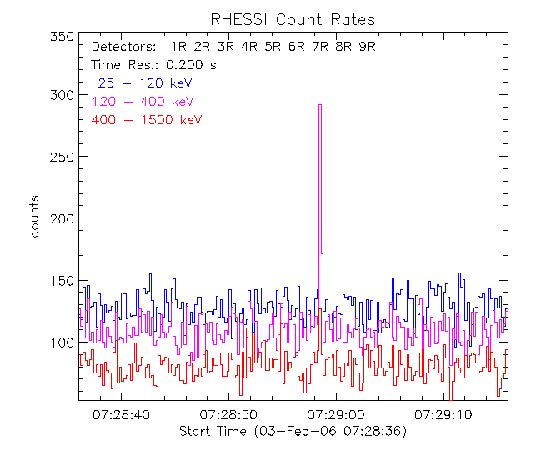
\includegraphics[scale=0.46]{Images/ipn_light_curve.png}
%\label{ipn_light_curve}
\end{minipage}
\hspace{0.5cm}
\begin{minipage}[b]{0.5\linewidth}
\centering
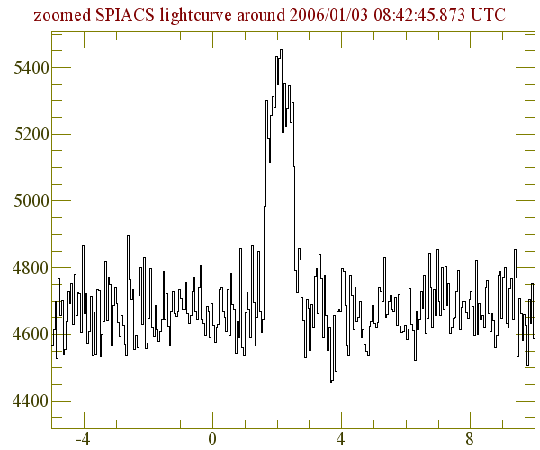
\includegraphics[scale=0.35]{Images/060103_flattop.png}
%\label{060103_flat}
\end{minipage}
\caption{(Left figure) Light curve for GRB060203 obtained using data from the RHESSI mission: gamma photons counts on the $y$--axis versus time in seconds on the $x$ axis; the photons are detected in three different energy bands: 25--120, 120--400, 400--1500 keV and we observe a narrow single peak in the medium energy band indicative of a (possible) short GRB. Image reproduced from \cite{heasarc}. Together with the short durations, light curves represent strong proofs of the short hard nature of the GRBs in the sample. (Right figure) Light curve for GRB060103 (120--400 keV band), displaying a somewhat flat top structure. The width is roughly 2 s wide and the peak is steep, good indicators for a short burst. Image reproduced from \cite{integral}.}
\label{two_light_curves}
\end{figure}

\section{Search Methodology}
\label{sec:method}

\subsection{Overview}
For the IPN short GRBs, the data streams from the operational detectors will be combined coherently and searched using the methods described in \cite{Harry:2010fr} and summarized in Chapter ~\ref{Chapter Three}. The search for compact binary coalescing signals is done using match filtering \cite{OwenSathyaprakash98} by correlating the detector data against theoretical waveforms that replicate the signal for a broad interval of binary parameters and are collected in a template bank, as described in Chapter \ref{Chapter Three}. These expected GW waveforms depend on the masses and spins of the NS and its companion (either NS or BH), as well as on the distance to the source, its sky position, its inclination angle, and the polarization angle of the orbital axis. The template bank used in the IPN GRB search is identical to the one used for the S6/VSR2 and 3 GRB search \cite{lvc:s6grb} and described in Chapter \ref{Chapter Four} with analysis theory described in Chapter \ref{Chapter Three}. 

The search identifies an ``on--source''  time in which to search for an associated GW event. In the compact binary coalescence model for short GRB progenitor, it is believed that the delay between the merger and the emission of gamma--rays will be small (references found in Chapter \ref{Chapter Two} and \ref{Chapter Three} and \cite{lvc:s6grb}). We therefore use an interval of 5 s prior to the GRB to 1 s following as the on--source window, which is wide enough to allow for uncertainties in the emission model and in the arrival time of the electromagnetic signal at the IPN spacecraft, as well as for the differences in sensitivity of the IPN detectors. As described in \cite{Predoi:2011aa} and Chapter \ref{Chapter Six}, the burst time of arrival at Earth was chosen to be the time of arrival at the IPN spacecraft nearest to Earth, usually located at less than 1 lightsecond and therefore the arrival time would have an uncertainty less than 1 s. 

It is important to mention, that for the IPN GRBs that have a time of arrival error larger than 1 s, i.e., the closest IPN spacecraft to Earth is further than 1 lightsecond, near--Earth satellites such as \emph{Swift}, RHESSI or Suzaku are used for timing refinement. Although these spacecraft do not participate effectively in the detection process for these bursts, they display a Recorded Increase (RI) in the photon count at the time of the burst. This is not above their GRB detection threshold but can be used for timing the burst. Namely, three short bursts have had their burst trigger time at Earth adjusted using data from \emph{Swift}, RHESSI or Suzaku: GRB070516 uses \emph{Swift} that triggers at 74484.661 s after the start of day, the refined trigger time will be GPS 863383298 with a precision of $<$1 s; GRB061006A uses RHESSI that refines the time to 31418.224s and Suzaku to 31417.698s (shift due to different sensitivities, i.e., both detectors observe the burst in different energy bands, with peaks at different times), the refined trigger time will be GPS 844159432 with a precision of $\approx$ 1 s; GRB060107 uses Suzaku detection in low time resolution at 06885.556$\pm$0.880 s, the refined time will be GPS 820634099 with a precision of $\approx$ 1.8 s. Also, two bursts have had their arrival time adjusted even if no near--Earth satellite was available, using a timing software provided by Kevin Hurley: GRB070222 with Earth crossing times software giving two possible values at 27115.112 s and 27117.161 s after the start of the day, refined time GPS 856164729 with a precision of 2 s; GRB060930A software analysis gives Earth crossing times at 09051.997 s and 09053.120 s, with a refined time at GPS 843618666 and a precision of 1 s.   

\subsection{Searching the error box}
The on--source data are analyzed by the search algorithms to detect possible GW transients, referred to as ``events''. The search for events is sensitive to sky location and will be done across the IPN GRB error box. We will generate a grid of search points to pave each GRB's error box in order to increase the chances of finding a signal over the entirety of the box. A fixed grid spacing (distance between adjacent grid points) of 1.8 degrees will be used for the search, motivated by the GW detectors' power of resolving the sky location, described in \cite{Predoi:2011aa}. Each error box is a 3--$\sigma$ region but we will search and assign equal detection probability to each search point. An example of an error box paved with search points can be seen in Figure \ref{ipn_search}. The analysis pipeline makes use of a single text file containing the equally--spaced search points for both the processing and post--processing stages. 

\begin{figure}[htb]
\begin{center}
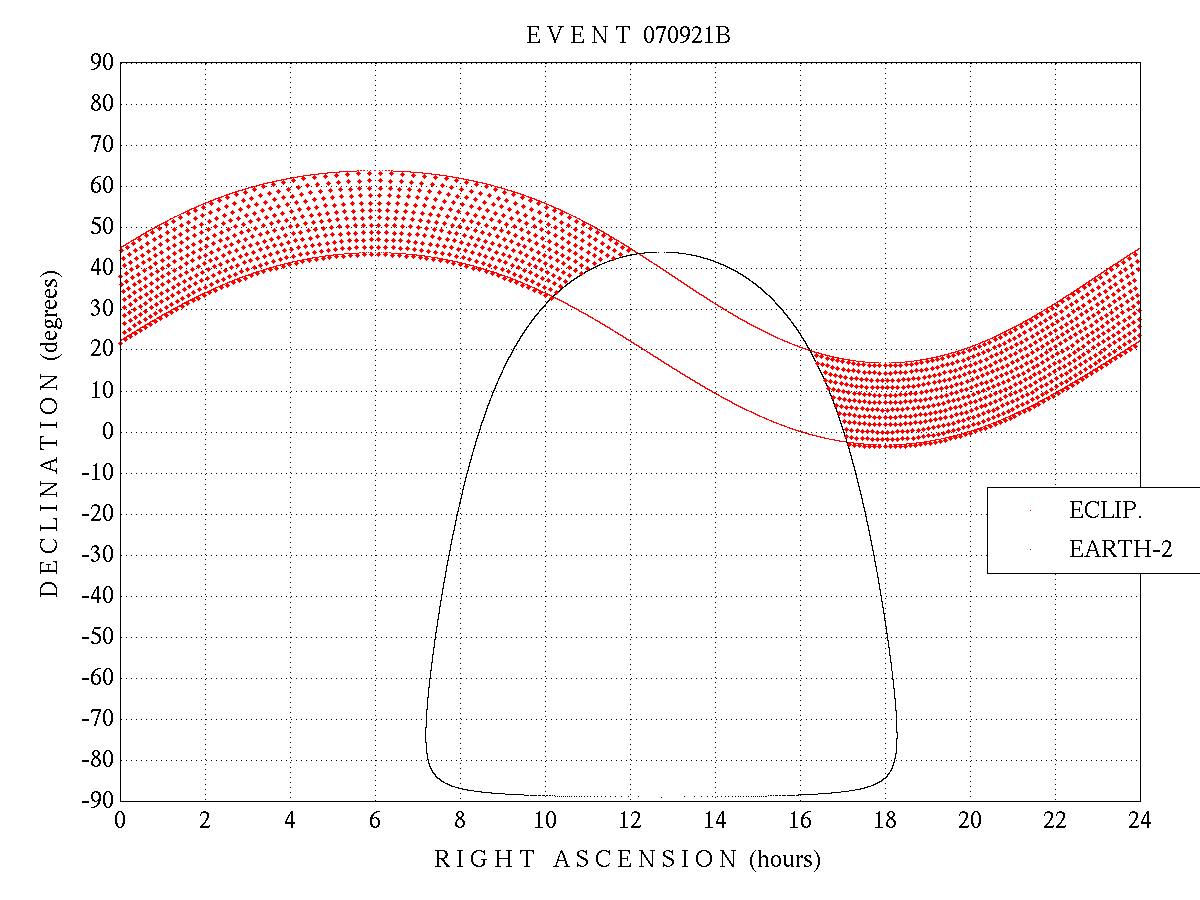
\includegraphics[width=32pc]{Images/ipn_search.png}
\caption{\label{ipn_search} A typical IPN GRB error box populated with search points: the search points are firstly distributed along the central line of the IPN annulus, at 1.8 degrees relative distance; if the annulus is wide enough to permit, a square 2--D grid with a 1.8$\times$1.8 degrees cell is built across the error box. This ensures an even search for signals. For illustration purposes only, we are showing the error box for GRB070921B, a long burst with a large error box, constructed from the intersection of Konus ecliptic band and Earth constraint; the error box contains a considerable number of search points.}
\end{center}
%\label{errorbox}
\end{figure}


The pipeline orders events found in the on--source time according to a ranking statistic described in \cite{Harry:2010fr} and Chapter \ref{Chapter Four}. In order to cope with the effects of non--stationary, transient noise ``glitches'' in the GW detectors' data, the pipeline uses a number of signal consistency tests, including the null stream, amplitude consistency and several $\chi^{2}$ tests \cite{Allen:2004gu, Harry:2010fr, Hanna:2008} and Chapter \ref{Chapter Four}. Also, candidate events are subjected to checks that ``veto'' events overlapping in time with known instrumental or environmental disturbances, see Chapter \ref{Chapter Four}. The surviving event with the highest ranking statistic is taken to be the best candidate for a gravitational wave signal for that GRB; it is referred to as the {\it loudest event} \cite{Brady:2004gt,Biswas:2007ni}. In order to estimate the significance of the loudest on--source event, the pipeline uses two background or ``off--source'' data segments on either side of the on--source, as described both in \cite{lvc:s6grb} and in Chapter \ref{Chapter Four}. Given this off--source segments' placing, it is assumed that the on--source and the off--source detector data have the same noise properties. To determine if a GW is present in the on--source data, the loudest on--source event is compared to the distribution of loudest off--source events. A false alarm probability (FAP) is defined as the probability of obtaining such an event in the on--source, given the background distribution, under the null hypothesis, as described in Chapter \ref{Chapter Four}, Chapter \ref{Chapter Five} and in \cite{lvc:s6grb}.

In the same manner as in the S6/VSR2 and 3 GRB search \cite{lvc:s6grb}, the pipeline efficiency of recovering signals is determined by performing simulations injected in the data. In the case of the IPN GRB search the simulations' parameters (masses, spins and inclinations) are identical to the S6/VSR2 and 3 GRB search: they are drawn from two sets of astrophysically motivated compact binary systems as GRB progenitors -- two neutron stars (NS--NS) and a neutron star with a black hole (NS--BH) for a set of four possible \emph{maximum} inclination angles (10$^\circ$, 30$^\circ$, 45$^\circ$ and 90$^\circ$).

In terms of simulated parameters, the NS masses are chosen from a Gaussian distribution centered at 1.4~$\mathrm{M_\odot}$ \cite{Kiziltan:2010ct,Ozel:2012ax} with a width of 0.2~$\mathrm{M_\odot}$ for the NS--NS case, and a broader spread of 0.4~$\mathrm{M_\odot}$ for the NS--BH systems, to account for larger uncertainties given the lack of observations for such systems. The BH masses are Gaussian distributed with a mean of 10~$\mathrm{M_\odot}$ and a width of~6\,$\mathrm{M_\odot}$. The BH mass is restricted such that the total mass of the system is less than $25\,M_{\odot}$. For masses greater than this, the NS would be ``swallowed'' by the BH, no massive torus would form, and no GRB would be produced \cite{Ferrari:2009bw,0264-9381-27-11-114002,lrr-2011-6}; the NS spins are uniformly drawn within the [0, 0.4] interval, the BH spins are uniformly drawn from the [0, 0.98) interval with a tilt angle $<~60^\circ$.

The simulated sky locations cover the entirety of the IPN GRB error box. To generate these positions, the error box is first paved with a symmetric grid of points with a 0.2 degree grid spacing. This is a finer spacing than the one which is used for the search to ensure efficient coverage of the error box by the simulated positions. It will also provide a verification that the 1.8$^{\circ}$ spacing of search points is adequate.  Random positions are generated within a small square bin centered at each of these grid points and whose sides have lengths equal to the grid spacing. The relative number (or density) of positions generated for each grid point is weighted according to the estimated source position probability distribution. The probability distribution that will be used in the case of a single 3--$\sigma$ IPN annulus is a one--dimensional Gaussian distribution centered at the central radius of the IPN annulus, and which has a sigma of 1/3 the width of the given annulus half--width. For error boxes which are formed by the intersection of two 3-$\sigma$ IPN annuli, the probability distribution will be a two--dimensional Gaussian, with distances measured from the two central radii of the two annuli. This assures that there are proportionally more simulations for those positions with larger probabilities of having a signal. The pipeline then draws random locations for injections from this list of simulation points. An example of an IPN GRB error box populated with simulated sky positions can be seen in Figure \ref{ipn_simulations}.

\begin{figure}[htb]
\begin{center}
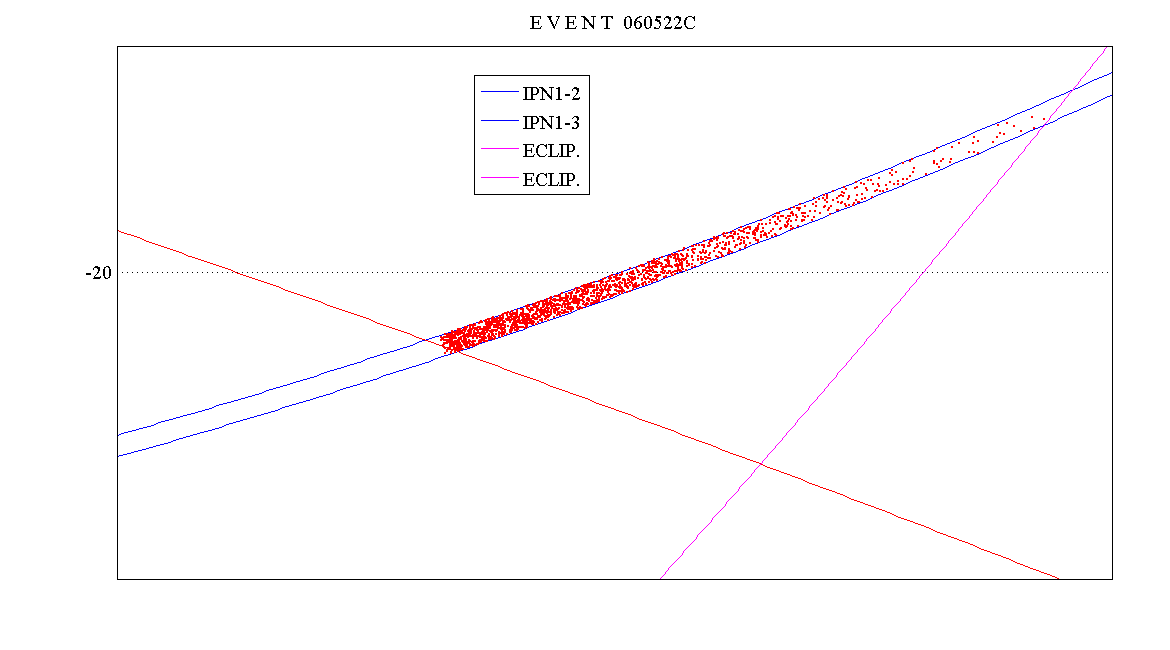
\includegraphics[width=32pc]{Images/ipn_simulations.png}
\caption{\label{ipn_simulations} A typical IPN GRB error box populated with simulation points: the simulation points are firstly distributed along the central line of the IPN annulus, at 0.2 degrees relative distance; a square 2--D grid with a 0.2$\times$0.2 degrees cell is built across the error box. Then simulation points are randomly thrown in each   bin centered at each point and sides equal to 0.2 degrees. The distribution of these points follows a 1-- or 2--dimensional Gaussian, depending on the number of IPN annuli: the width of the distribution corresponds to the width of the IPN annulus so that there are proportionally more simulation points thrown towards the center line of the annulus where the signal is expected to be found. In the case of two annuli, the 2--D Gaussian has the widths of the two IPN annuli. Here we see the distribution of simulation points for two intersecting IPN annuli, for GRB060522C, a short hard burst: there are more points towards the center of the intersection region and less towards the outer edge; the narrow IPN annulus intersecting the wider one will allow for an assymetric 2--D Gaussian distribution of simulation points, with more throws inside the narrow annulus and less inside the wider one.}
\end{center}
%\label{errorbox2}
\end{figure}

\subsection{Single chirp mass bin [0,8.0) $M_{\odot}$}

Another of the changes to the standard S6/VSR23 GRB analysis pipeline was introducing a single chirp mass bin for both off--source and on--source events. Both the S5/VSR1 and the S6/VSR23 GRB analyses used three chirp mass bins to bin both background and simulated events and calculate false alarm probabilities for on--source events (see Chapter \ref{Chapter Four} for an explanation for chirp mass binning). Binning was done in $\mathcal{M} \subset$[0, 3.48), [3.48, 6) and [6, 20) ~$M_{\odot}$ as we have already seen in Chapter \ref{Chapter Four}. The reason for chirp mass binning is that due to the large variation in the length of the templates used during the search (shortest template is $\approx$0.3 s and longest is $\approx$45 s), there is a larger variation in the templates responses to noise glitches in the detectors where glitches tend to match higher mass templates (and shorter), the result being triggers with larger values of SNR. The result is that in the high chirp mass bin we end up with very few and very loud (SNR before signal--based cuts, relatively to the other two bins) triggers and almost to none injections.

We constructed a simple plot of SNR vs. $\mathcal{M}$ for a test GRB shown in Figure \ref{chirptest}. In the figure, the grey (red) population represents triggers from noise and the black population represents the injections. We can see that beyond $\mathcal{M}=8~M_{\odot}$ noise triggers dominate the populations. This has been done after a glitch--rejection test had been applied prior to the chirp mass restriction: the glitch--rejection test asks for the detection statistic of any background trigger within 0.1 s of injected signal time to be larger than 95\% of the detection statistic of the recovered injection. As we can see in Figure \ref{chirptest}, the chirp mass restriction will remove any simulation spuriously identified with glitches and a number of loud background triggers.

\begin{figure}[htb]
\begin{minipage}{0.5\linewidth}
\centering
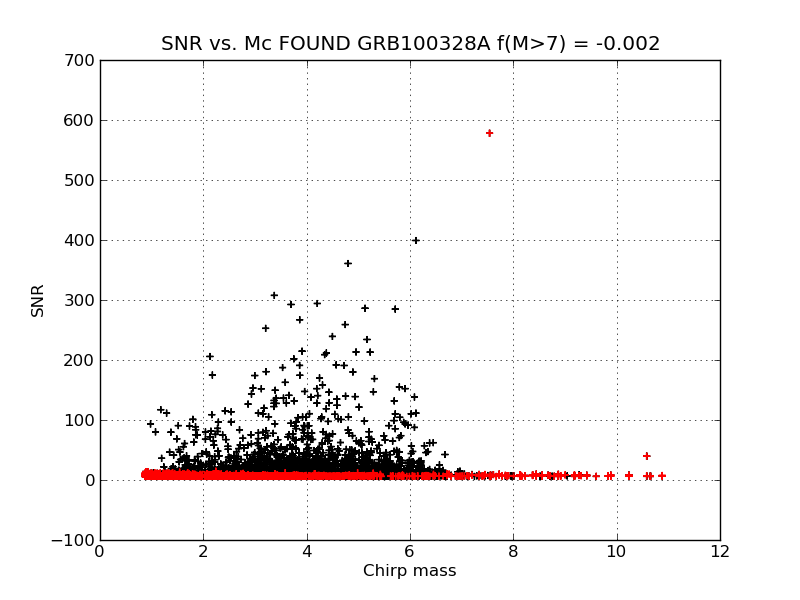
\includegraphics[scale=0.35]{Images/snr_mchirp.png}
%\label{snr_mchirp}
\end{minipage}
\hspace{0.5cm}
\begin{minipage}{0.5\linewidth}
\centering
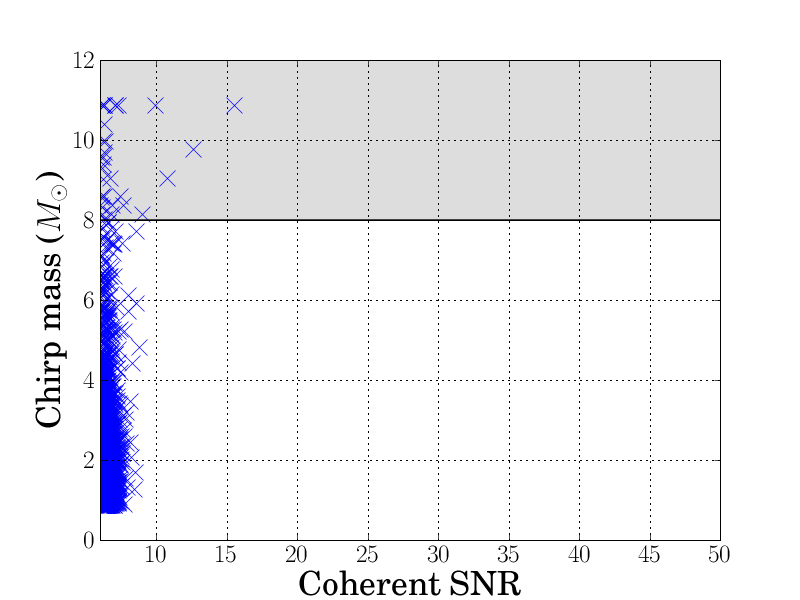
\includegraphics[scale=0.35]{Images/chirptest.png}
%\label{chirptest}
\end{minipage}
\caption{(Left figure) Noise triggers (red) and simulations triggers (black) in an SNR--$\mathcal{M}$ diagram for an example GRB analysis. This clearly shows that the population of triggers with $\mathcal{M}>8.0$ is dominated by noise (with the exception of a very loud glitch with SNR$\approx$575 and chirp mass just below 8). A limit on chirp mass 8.0 was thereafter used in the IPN GRB search. (Right figure) Background events shown in a coherent SNR -- chirp mass diagram; here an example where a set of loud background glitches were removed based on their chirp mass (the loud glitch from left plot is beyond the SNR scale).}
\label{chirptest}
\end{figure}

\subsection{Distance exclusion}
The further a GW source is, the weaker its signal at the detectors, as seen in Chapter \ref{Chapter One}, the GW amplitude scales with $1/D$. Therefore the pipeline is efficient in recovering signals up to a certain distance limit that depends on the sensitivity of the detectors at the time of the search. We would want to quote this limit and argue that if there was a GW source placed within this limit, we would have detected it. Whenever no statistically significant signal is found, a 90\% confidence level lower limit on the distance to the GRB progenitor (for both NS--NS and NS--BH merger models) is set. The quoted exclusion distances are marginalized over systematic errors that are inherent in this analysis: errors introduced by the mismatch of a true GW signal and the waveforms used in the simulations \cite{Abbott:2009tt} and amplitude errors from the calibration of the detector data \cite{Abadie:2010px}.

The GW signal exclusion distances are calculated for the four astrophysically--motivated opening angles that we performed our injections with (10$^\circ$, 30$^\circ$, 45$^\circ$ and 90$^\circ$). The steps taken to obtain the exclusion distance are as follows:

\begin{itemize}
\item
Determine the loudest event in the on--source in the single searched chirp mass bin;
\item
For each injection we find the trigger with the loudest SNR within 0.1 s (NOTE: loudest SNR and NOT loudest value of detection statistic) and associate this trigger with the injection. If there are no triggers within 0.1 s the injection has no trigger associated to it and will be considered ``missed'' for all purposes. NOTE: an injection will have either 1 or 0 triggers associated to it;
\item
Calculate the value of the detection statistic for the found trigger;
\item
If that value is less than the loudest onsource trigger the injection is marked as ``missed'' for distance exclusion purposes; for any injection whose found trigger is louder than the on--source event, we look at the 0.1 s around the time the injection was made. We find the loudest trigger in the off--source (if there is no trigger the injection is marked as ``found''). We compare the value of the detection statistic for this trigger with the injection's trigger. If the injection trigger is $>1.1~\times$ louder than the offsource trigger, the injection is marked as ``found'', if not the injection is marked as ``missed'' -- this is because all injections, as loud signals, are supposed to be louder than any of the background triggers; 
\item
We then bin the injections in distance and calculate the fraction of injections that are ``found'' as a function of distance. An example is shown in Figure ~\ref{distance_excl_stats};
\item
We then read off the distance at which the efficiency drops below 90\% and quote that as the 90\% exclusion distance.
\end{itemize}

\begin{figure}[htb]
\centering
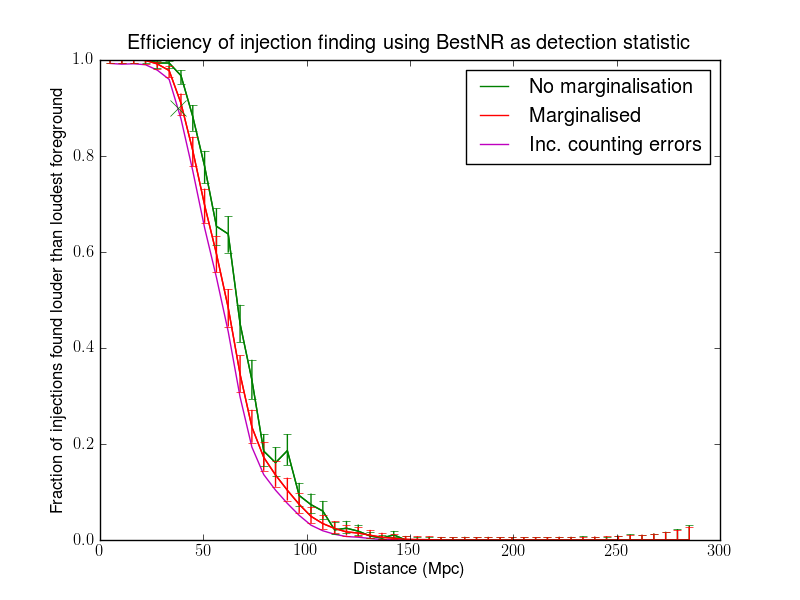
\includegraphics[width=28pc]{Images/distance_excl_stats.png}
\caption{The efficiency of finding injections as a function of distance to the source (percentage of ``found'' injections vs. distance). The pipeline is considered efficient up to an injection recovery percentage of 90\%, limit that gives us the confidence level lower limit on the distance to the GRB progenitor, here 37.6 Mpc. The green curve is un--marginalized, the red one is marginalized over the waveform and calibration errors, and the pink one includes counting (binomial) errors as well (since we did only a finite number of injections).}
\label{distance_excl_stats}
\end{figure}

\subsection{H1H2--only GRBs}

The analysis for the six GRBs that have data from H1H2--only is similar to the other 14 (12 presented here) multiple detectors GRBs with a few changes. Since H1 and H2 are co--located and co--aligned, there is no sensitivity to sky--location and the search will be done at a single sky point. It is irrelevant how we choose this point, as long as it is inside the GRB positional error box. Simulations will be performed across the whole error box, just as in the other GRB's case. A typical large error box for an H1H2--only GRB is shown in Figure \ref{h1h2_ipn_simulations}. The analysis will need tuning for a precise way of computing the different null--stream and $\chi^2$ veto tests, due to the particular nature of the GW detectors used. This work is in progress at the time of writing and will be finished shortly.

\begin{figure}[htb]
\begin{center}
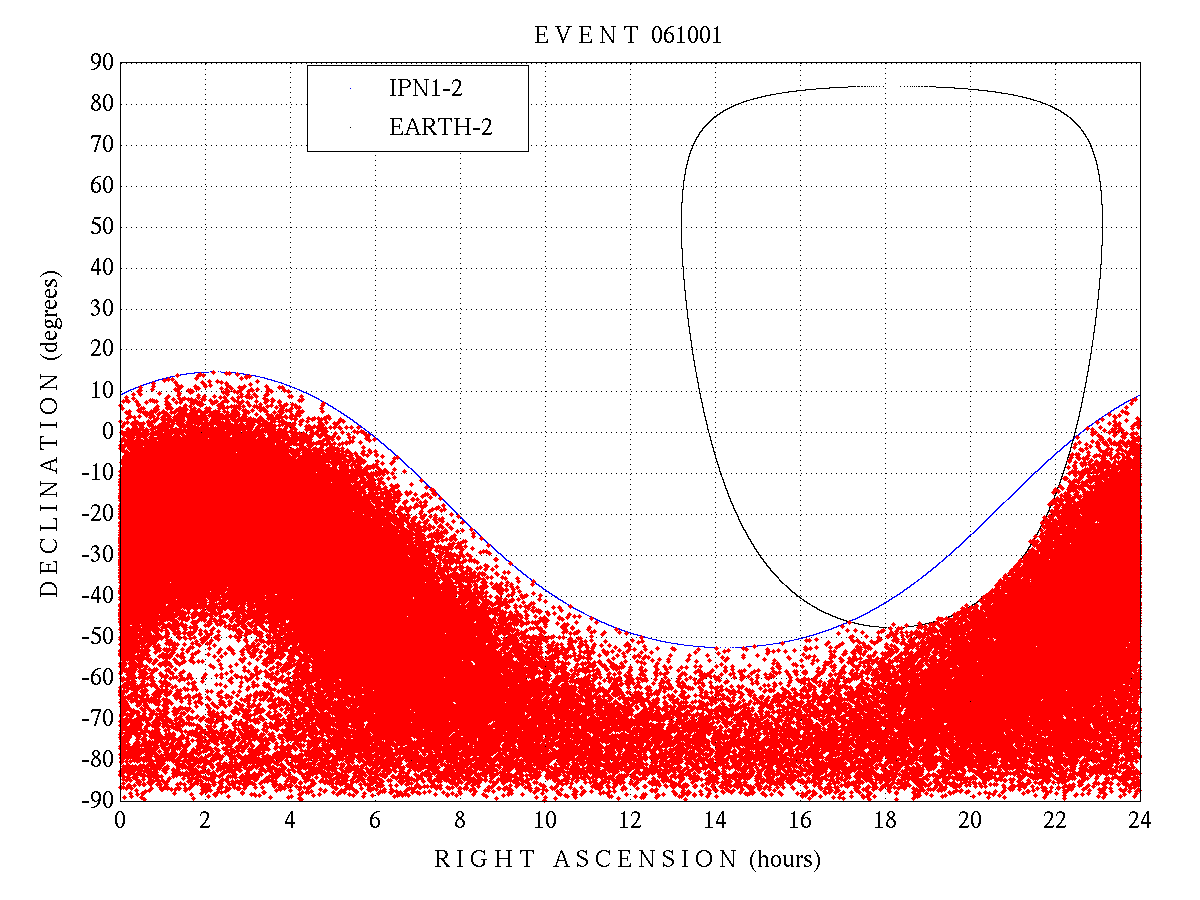
\includegraphics[width=28pc]{Images/GRB061001_simulations.png}
\caption{\label{h1h2_ipn_simulations} A typical H1H2--only IPN GRB large error box populated with simulation points (here the short hard burst GRB061001): a large error box is constructed by the intersection of a single IPN annulus and Earth constraint, and populated with simulation points, with more points towards the center and less towards the edges of the error box.}
\end{center}
\end{figure}

\subsection{GRB090802A, a testbed for the IPN analysis}

GRB090802A was the only three--detector (with data available from Hanford H1, Livingston L1 and Virgo V1 GW detectors) Fermi--GBM short GRB with a trigger time during S6/VSR23 and its positional error box was refined using data from the IPN. As such, this GRB was a testbed for the analysis changes specific to the search around the times of short bursts localized by the IPN. It was also the first time that a GW search prompted a GRB observers team (Fermi--GBM) to update an official but previously obsolete sky position (shown in Figure \ref{090802_IPN} together with the IPN localization) for the sole purpose of a GW analysis; as a result of changes in the codes that calculate the Fermi--GBM GRB rates, the initial sky position of GRB090802A was shifted by $\approx30^{\circ}$. The positional error box is shown in Figure \ref{090802_IPN} and was obtained from the intersection of two IPN annuli (triangulated using timing information from Konus--WIND, INTEGRAL and Fermi--GBM) and the Fermi--GBM 3--$\sigma$ error contour.

\begin{figure}[ht!]
\begin{minipage}{0.5\linewidth}
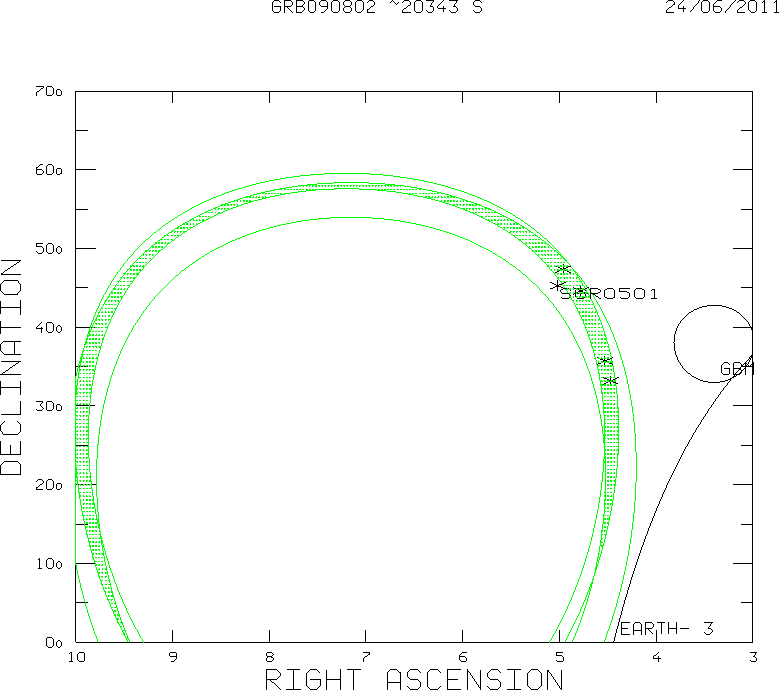
\includegraphics[scale=0.35]{Images/090802EB_IPN.png}
\end{minipage}
\hspace{0.5cm}
\begin{minipage}{0.5\linewidth}
\centering
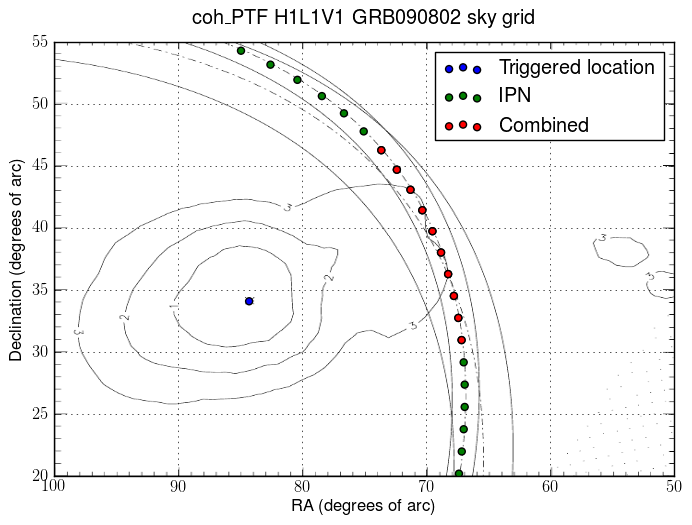
\includegraphics[scale=0.41]{Images/090802_eb.png}
\end{minipage}
\caption{(Left figure) GRB090802A: IPN localization (intersection of two IPN annuli, green shaded region) and initial Fermi--GBM error box (right small circle), with Earth constraint visible on the right; the GBM localization was shifted as a result of reprocessing the data to a final position shown on the right. Right ascension (RA) in hours and declination (dec) in J2000 degrees (courtesy of Kevin Hurley). (Right figure) GRB090802A: positional error box and GW search points. The error box is the result of the intersection of two IPN annuli (triangulated using timing information from Konus--WIND, INTEGRAL and Fermi--GBM; shown here with continuous line and center radii with dashed lines) and the Fermi--GBM 3--$\sigma$ error contour (the irregular shape, approximated with a systematic errors circle with a radius 4.9 degrees). The red points represent the GW search points.}
%\end{minipage}
\label{090802_IPN}
\end{figure}

The analysis for this GRB used the same procedure of paving an extended error region with search and simulation points as in the IPN GRB case, as described above. The full results of the data analysis associated with GRB090802A can be found in \cite{lvc:s6grb}.

\section{Significance of FAP population}
\label{sec:fappop}

We use a weighted binomial test to assess whether the obtained set of FAPs is compatible with the uniform distribution expected from noise only. This test looks for deviations from the null hypothesis in the 25\% tail of lowest FAPs weighted by the prior probability of detection (estimated from the GW search sensitivity). The weighted binomial test is identical to the one used for the S6/VSR2 and 3 GRB analysis \cite{lvc:s6grb}. The test weighs more the GRBs that have a larger prior probability of detection, hence with more chances for a GW detection. The details of this test are given in \cite{lvc:s6grb} and briefly described below.

The IPN GRB analysis was done for every GRB in the sample, independently one from another. Since there was no detection made for any of the bursts, a non--detection test is necessary: the individual analysis of each GRB rules out the detection of a loud signal but does not exclude a population of weak GW signals. This test accounts for any individual deviation from the background distribution or for a collective presence of a weak gravitational wave signal. The binomial test considers the set $\{p_i\}_{1 \leq i \leq  N_\text{GRB}}$ of false alarm probabilities (FAPs) obtained for a population of $N_\text{GRB}$ analyzed GRBs, sorted increasingly. The smallest $N_\text{tail} = 0.25 N_\text{GRB}$ of these FAPs are used to search for an excess of weak signals. The binomial probability, under the no--signal hypothesis, of obtaining at least $k$ events with FAPs less than the actual $k$--th FAP $p_k$ is calculated for $1 \leq k \leq N_\text{tail} $ and the minimum of these probabilities is used as a detection statistic:
%
\begin{equation}
S_\text{binomial} =  -\log \min_{1\leq k \leq N_\text{tail}} \sum_{l\geq k} \binom{N}{l} p_k^l
  (1-p_k)^{N-l} \, .
\end{equation}
%
$S_\text{binomial}$ looks for a deviation of the FAP distribution when compared to the uniform distribution of FAPs expected from background, in the low FAP region where an excess of weak gravitational wave signals might be present. 

In order to account for the contribution of GRBs for which the GW detector sensitivity is poor we construct a weighted binomial test that is based on a statistic that depends now on the \emph{a priori} GW detection probabilities: the sensitive volumes of the GW search associated with each GRB trigger, which depends on the GRB sky position and the performance of GW detectors at the time of the search \cite{lvc:s6grb}. This is as follows:
%
\begin{itemize}
\item Based on the background and sensitivity to simulated signals, compute the
  distance $d_k(m)$ at which the detection efficiency is equal to 50\%
  for GRB $k$ and signal emission model $m$ (either NS--NS or NS--BH coalescences).
\item Compute the relative volume ratio $R_k(m) = d_k(m)^3/\max_k
  d_k(m)^3$ for model $m$ compared to the most sensitive GRB.
\item Average the relative volume ratio over the different models
  $R_k = \textrm{mean}_{m} R_k(m)$.
\item Consider the penalized FAPs $p_k/R_k$ sorted in increasing
  order, and compute the detection statistic
  \begin{equation}
    S_\text{weighted} = -\log \min_{1\leq k \leq N_\text{tail}} 
  \binom{N}{k}\prod_{l \leq k}\frac{p_l}{R_l} \, .
  \end{equation}
\end{itemize}

The result of the weighted binomial test is a single ranking statistic  $S_\text{weighted}$.  The statistical significance of the measured $S_\text{weighted}$ is assessed by comparing to the background distribution of this statistic from Monte Carlo simulations with FAPs uniformly distributed in $[0,1]$. This yields the overall background  probability of the measured set of FAPs.

\section{Results}
\label{sec:results}

The distribution of FAP values for each of the 12 short IPN GRBs analyzed is shown in Figure \ref{fig:binomialTestCBC}. The result of the weighted binomial population detection test yields a background probability of $\approx$99\%, corresponding to an almost--perfect match with the no--signal hypothesis. In conclusion, no noteworthy individual events were found by this search, nor a collective presence of weak gravitational signals.

\begin{figure}[htb]
\centering
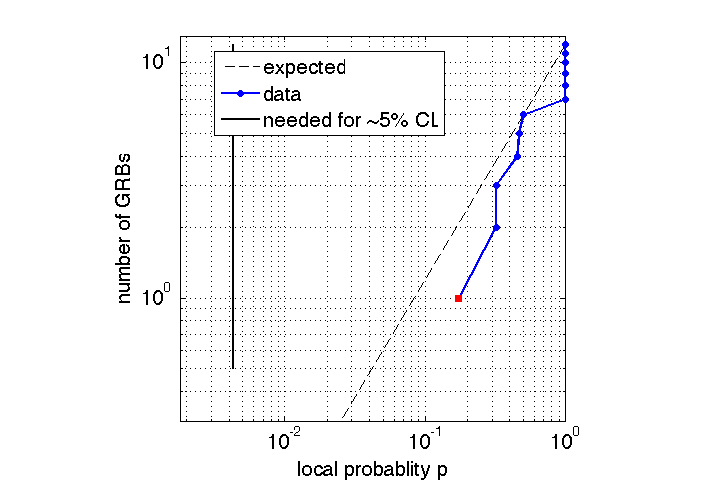
\includegraphics[width=28pc]{Images/binomial_test.png}
\caption{Cumulative FAP distribution from
the analysis of 12 IPN GRBs. The expected
distribution under the no--signal hypothesis is indicated by the
dashed line.}
\label{fig:binomialTestCBC}
\end{figure}

Given that no significant event was found in our analysis, we place upper limits on GW emission based on the signal models for short hard GRBs, discussed in Chapter \ref{Chapter Two} and \cite{lvc:s6grb} (short hard GRBs are commonly accepted to have either NS--NS or NS--BH mergers as progenitors). We will also compare these results with the GW detector sensitivity estimates during S5/VSR1.

For each GRB we derive a 90\% confidence lower limit on the distance to the GRB progenitor for either an NS--NS or NS--BH merger model, assuming a jet half--opening angle of 30$^\circ$. The distance limits are given in Table ~\ref{tab:ipn_grb_results} for each IPN GRB and a histogram of their values is shown in Figure ~\ref{fig:dist_insp}. The median exclusion distance for NS--NS is 18 Mpc and for NS--BH is 31 Mpc for the 30$^\circ$ jet cone. Fig.~\ref{fig:dist_excl_opening} and Table \ref{excl_dist_angles} show the median exclusion distances for half--opening angles of 10$^\circ$, 30$^\circ$, 45$^\circ$, and 90$^\circ$. The amplitude of a GW signal is stronger for smaller jet--opening angles and the excluded distances to progenitors are larger, whereas for large opening angles, the signal is weaker and the power of exclusion is much lower, as there are orientations which will give very little observable GW signal in the detector network. We can compare these results with the detectors' sensitivity measured by the inspiral horizon distance (see Chapter \ref{Chapter Three} for definition): during S5/VSR1 for a 1.4--1.4 $M_{\odot}$ binary the inspiral horizon distance was $\approx$35 Mpc and for a 5.0--5.0 $M_{\odot}$ binary the inspiral horizon distance was $\approx$70 Mpc for the most sensitive detectors (H1 and L1) (see Figure \ref{rangevmass}). Given that the inspiral horizon distance is calculated for an optimally--oriented binary, and the IPN GRBs have different orientations, we would expect the median exclusion distance to be reduced by a factor of two from the horizon distance (an approximate explanation for this is that the range is roughly half the horizon distance for all--sky events; in the GRB case we have nearly face--on events but only 90\% upper limits, therefore giving a factor of order 2). In turn, quoting the exclusion distances for the 22 \emph{Swift} GRBs during S5/VSR1, the median exclusion distance for an NS--BH system was 7 Mpc and for an NS--NS system was 3 Mpc \cite{Abadie:2010uf}. However, a direct comparison of the IPN and S5/VSR1 exclusion distances can not be established for a number of reasons: the S5/VSR1 analysis made use of the H1H2 pair of detectors with H2 roughly twice less sensitive than H1 or L1; the exclusion distances were calculated in a different manner during S5/VSR1 (see \cite{Abadie:2010uf} for method details).
 

\begin{figure}[htb]
\centering
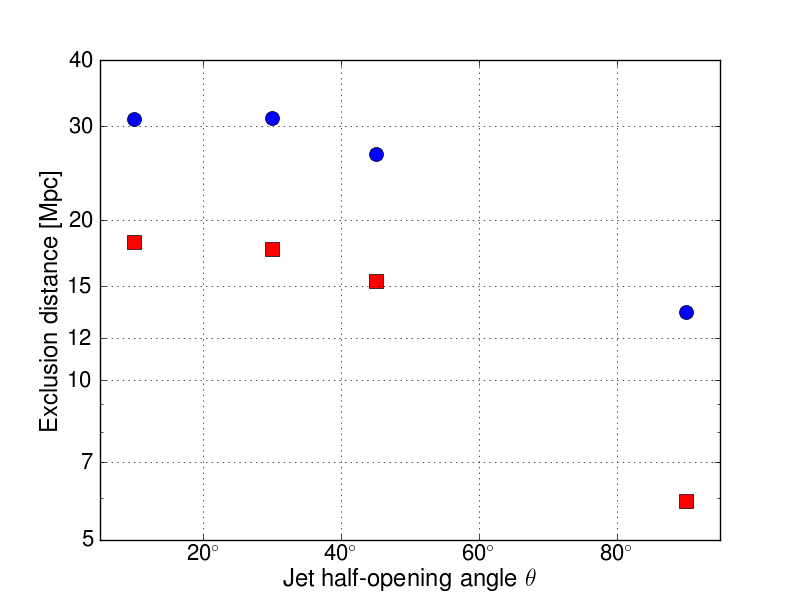
\includegraphics[width=26pc]{Images/figure_CBCexclusion_openingangle_points.png}
\caption{Median exclusion distances of CBC sources as a function of
half-opening angle, sampled at 10$^\circ$, 30$^\circ$, 45$^\circ$, 
and 90$^\circ$.  The medians are computed over the set of 12 analyzed short IPN GRBs, 
for both NS--NS and NS--BH, at 90\% confidence level.}
\label{fig:dist_excl_opening}
\end{figure}

\begin{table}[htb]
\begin{center}
\begin{tabular}{*{3}{l}}
\hline
Opening Angle & Dist. NS--NS (Mpc) & Dist. NS--BH (Mpc) \\
\hline
10 & 18.2 & 31.0 \\
30 & 17.6 & 31.1 \\
45 & 15.4 & 26.6 \\
90 & 5.9 & 13.4 \\
\hline
\end{tabular}
\caption{Exclusion distances for four different jet opening angles $\theta$ for the two astrophysically--motivated short GRB progenitor models: binary NS or NS--BH; for the NS--NS case the median distance (at $30^\circ$ jet opening angle) is 18 Mpc; for the NS--BH case the median distance (at $30^\circ$ jet opening angle) is 31 Mpc.}
\label{excl_dist_angles}
\end{center}
\end{table}

\begin{figure}[ht!]
\centering
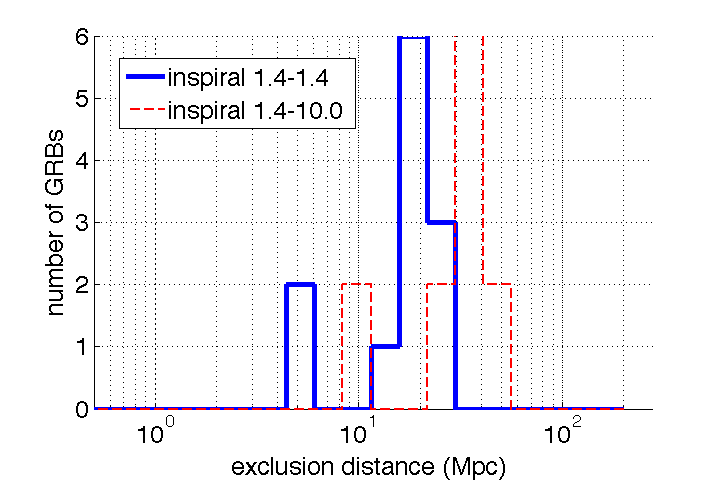
\includegraphics[width=28pc]{Images/dist_insp.png}
\caption{Histograms across the sample of short GRBs of the
distance exclusions at the 90\% confidence level for
NS--NS and NS--BH systems. See Table \ref{tab:shortGRB} 
for the exclusion values for each short GRB.}
\label{fig:dist_insp}
\end{figure}

\section{Possible host galaxies for two of the IPN GRBs}

Since the IPN GRBs have not been followed--up in X--ray and/or optical bands (due to extensive time delays in localizing them based on information from multiple IPN missions and due large positional errors), no afterglow has been detected in association with any of the bursts, therefore no galaxy host could be identified with sub--arcsecond precision. It is only natural to try and investigate any possible overlaps of their error boxes with nearby galaxies' error regions (at distances $<$40 Mpc). We did this using the Gravitational Waves galaxy catalog (GWGC). The GWGC is a new catalog of galaxies within 100Mpc, designed to be used in follow--up searches of optical counterparts from gravitational wave triggers. The catalogue contains up--to--date information compiled from the literature on sky position, distance and other astronomical parameters for more than 53,000 galaxies \cite{gwgc, White:2011qf}

Of the examined overlaps for each of the IPN short burst sample, two GRBs stand out with GW search points at very small RA--dec differences from the position of two nearby galaxies: GRB070414 error box overlapping PGC004601 (Andromeda II) and GRB070321 error box overlapping NGC5878, see Figure \ref{ipngrb_galaxies}.

\begin{figure}[htb]
\begin{minipage}{0.45\linewidth}
\centering
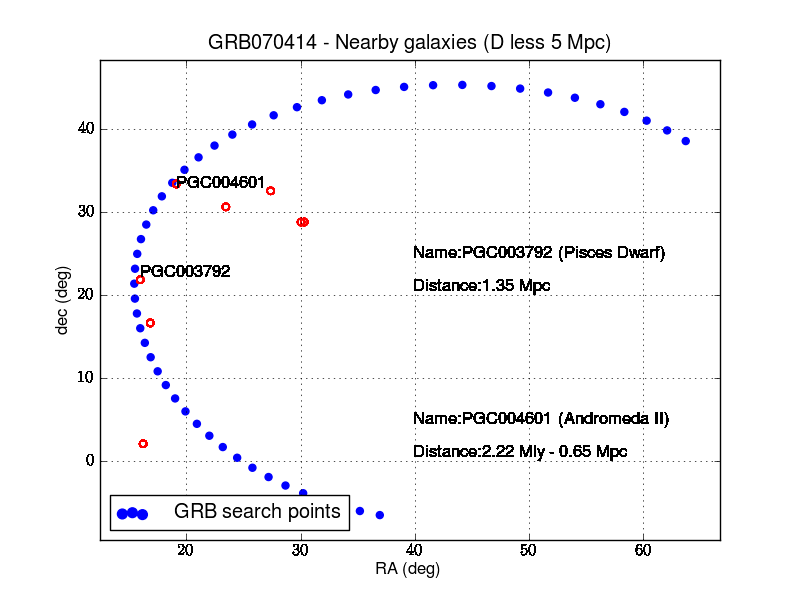
\includegraphics[scale=0.4]{Images/070414_andromeda2.png}
%\label{070414_andromeda2}
\end{minipage}
\hspace{0.5cm}
\begin{minipage}{0.40\linewidth}
%\begin{figure}[htb]
\centering
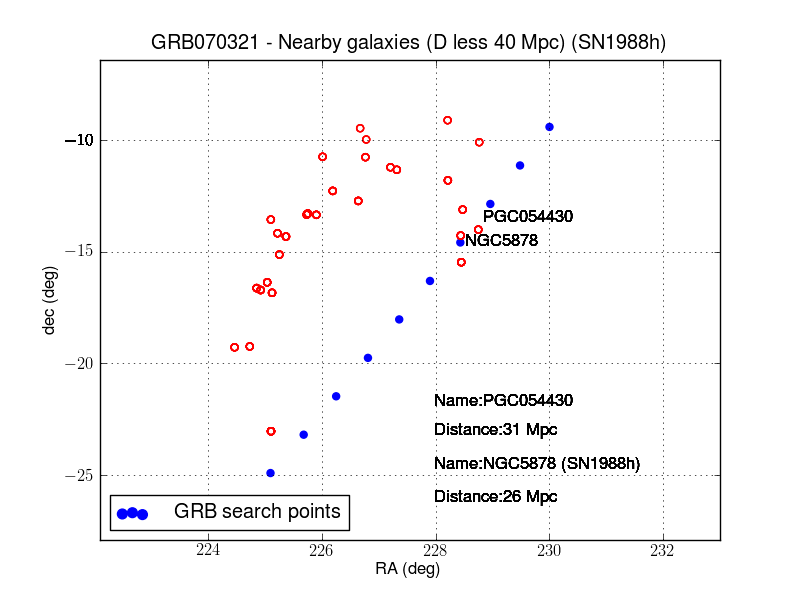
\includegraphics[scale=0.4]{Images/070321_galaxies.png}
\end{minipage}
\label{ipngrb_galaxies}
\caption{(Left figure) GRB070414 search points and nearby galaxies. Full circles represent the GW search points and empty circles represent galaxy locations, with $x$--axis RA and $y$--axis dec in J2000d degrees. Galaxy positions obtained from \cite{gwgc}. (Right figure) GRB070321 search points and nearby galaxies. Full circles represent the GW search points and empty circles represent galaxy locations, with $x$--axis RA and $y$--axis dec in J2000d degrees. Galaxy positions obtained from \cite{gwgc}}
%\end{minipage}
\end{figure}

An interesting case is that of GRB070414 whose IPN positional error box marginally overlaps the error box of a nearby galaxy, PGC004601 or Andromeda II, a dwarf spheroidal galaxy that is part of the Local Group and is a satellite galaxy of Andromeda M31. The distance to PGC004601 is $\approx$700 kpc (680$\pm$20 kpc). The GRB070414 has an extended, but very narrow error box with of $\approx0.3~\mathrm{deg}^2$, but the search point at RA=18.7719194, dec=33.5563965 degrees is situated only $\delta \approx$0.36 degrees from the center of the galaxy (equatorial position RA=19.12407, dec=33.41910 degrees (J2000d) \cite{ned}), as seen in Figure \ref{ipngalaxies_search_point}, and the IPN annulus intersects the outer region of the galaxy. The search point is quoted here just as a positional reference of the GRB error box median axis with respect to the galaxy error box; its position is arbitrary along the median axis, within the GRB error box, and depends entirely on how we chose to pave the error region with search points.

Another interesting case is that of GRB070321 whose positional error box neighbors the error region of galaxy NGC5878. The equatorial position of NGC5878 is RA=228.440458, dec=-14.269833 degrees (J2000d) \cite{gwgc,ned} and the nearest GW search point is located at RA=228.4346539, dec=-14.5788967 degrees giving us an RA--dec distance of only 0.31 degrees between the search point and the center of the galaxy. NGC5878 is located at a distance of 26.1$\pm$1.8 Mpc or redshift $z$=0.006641$\pm$0.000007, Local Group standard, and is a spiral galaxy of the same class as Andromeda M31 (SA(s)b \cite{ned}). The galaxy was host for a supernova event, SN1988H, a type II supernova that peaked in luminosity in February 1989 \cite{Cappellaro:1995ht}. Given the analysis results for GRB070321, we exclude a NS--BH merger within 36 Mpc with 90\% confidence.

Given the very low redshift of these two possible GRB host galaxies and the extended error regions of the GRBs, it is highly unlikely that the galaxies are indeed hosts for the bursts; even if, in fact, short GRBs are found closer in distance than long GRBs (see Chapter \ref{Chapter Two}), none of the short bursts with secured redshift measure has been observed at such low redshifts.

\begin{figure}[ht!]
\begin{minipage}{0.4\linewidth}
\centering
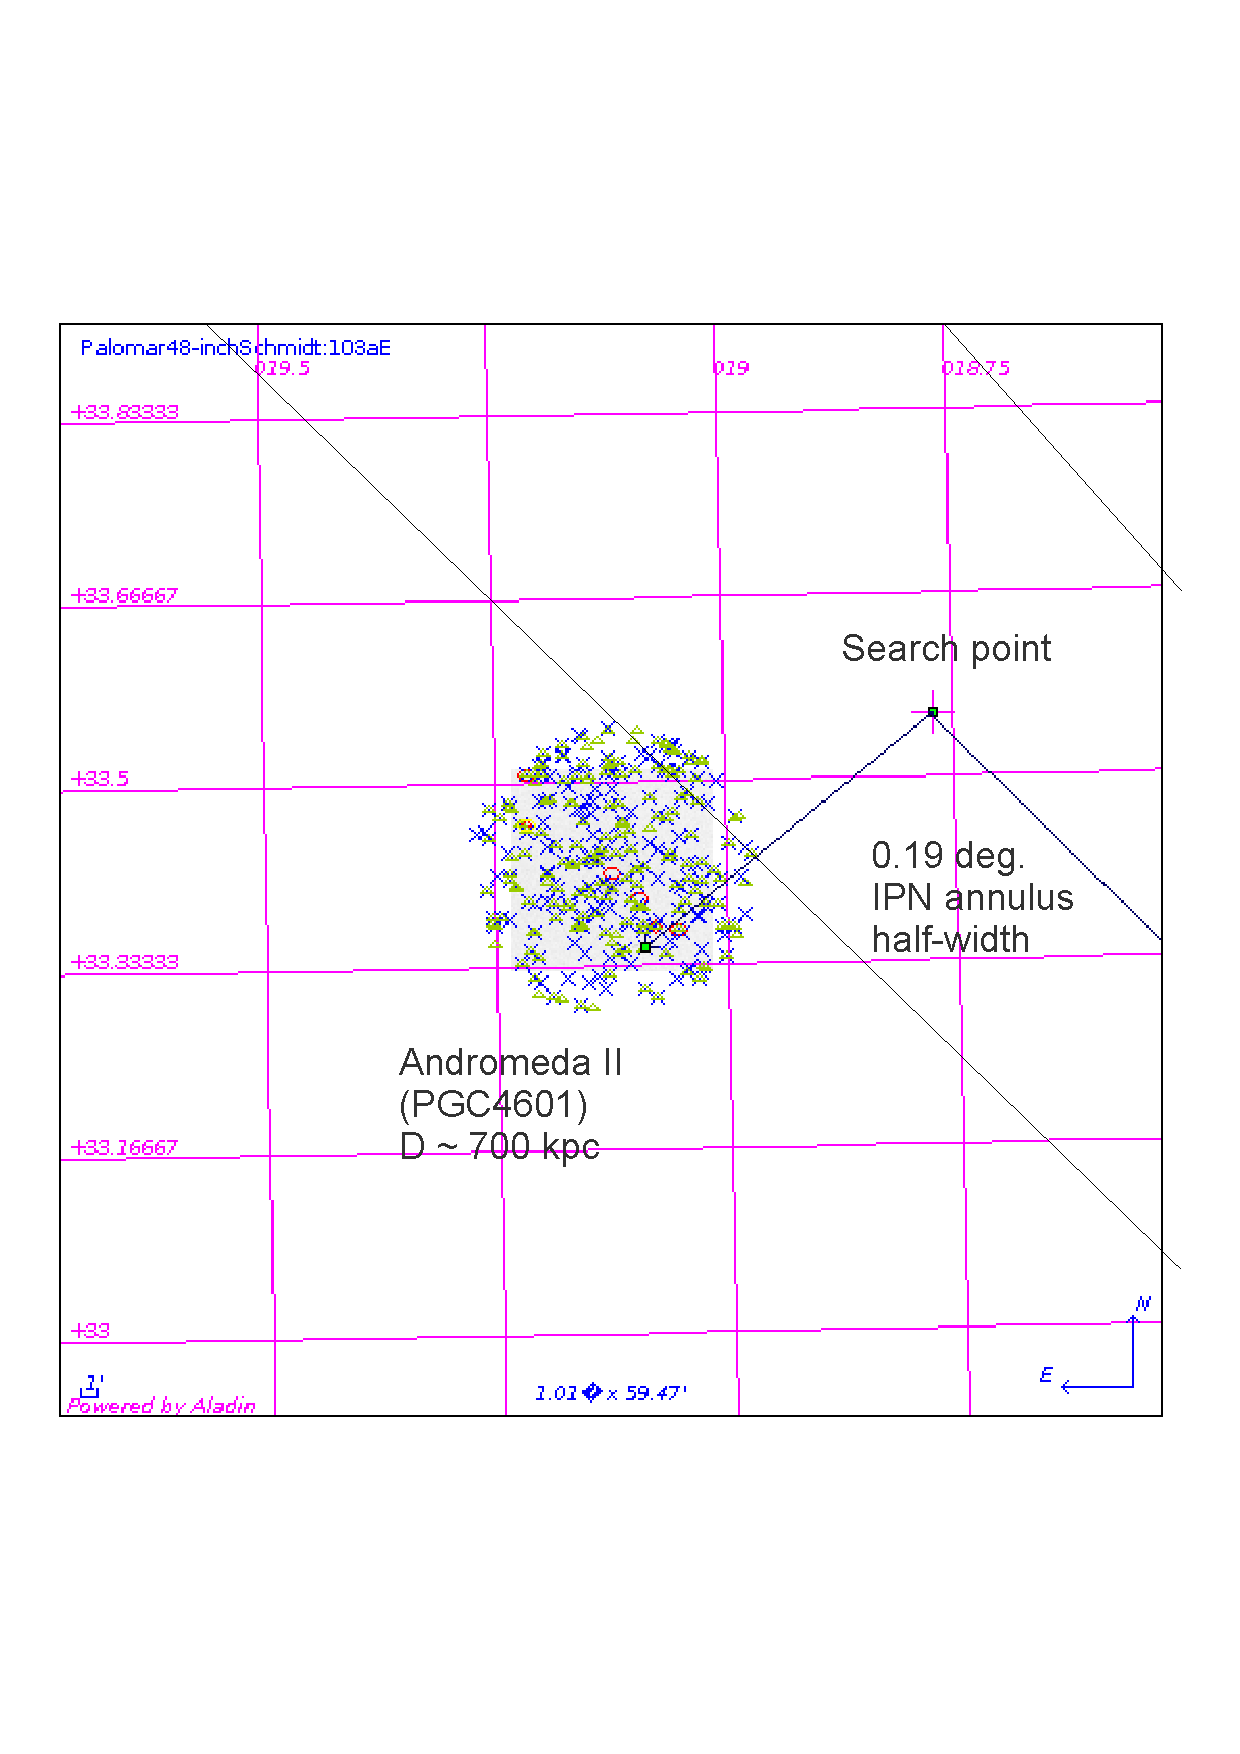
\includegraphics[scale=0.415]{Images/andromeda2.pdf}
%\label{andromeda2}
\end{minipage}
\hspace{0.5cm}
\begin{minipage}{0.5\linewidth}
\centering
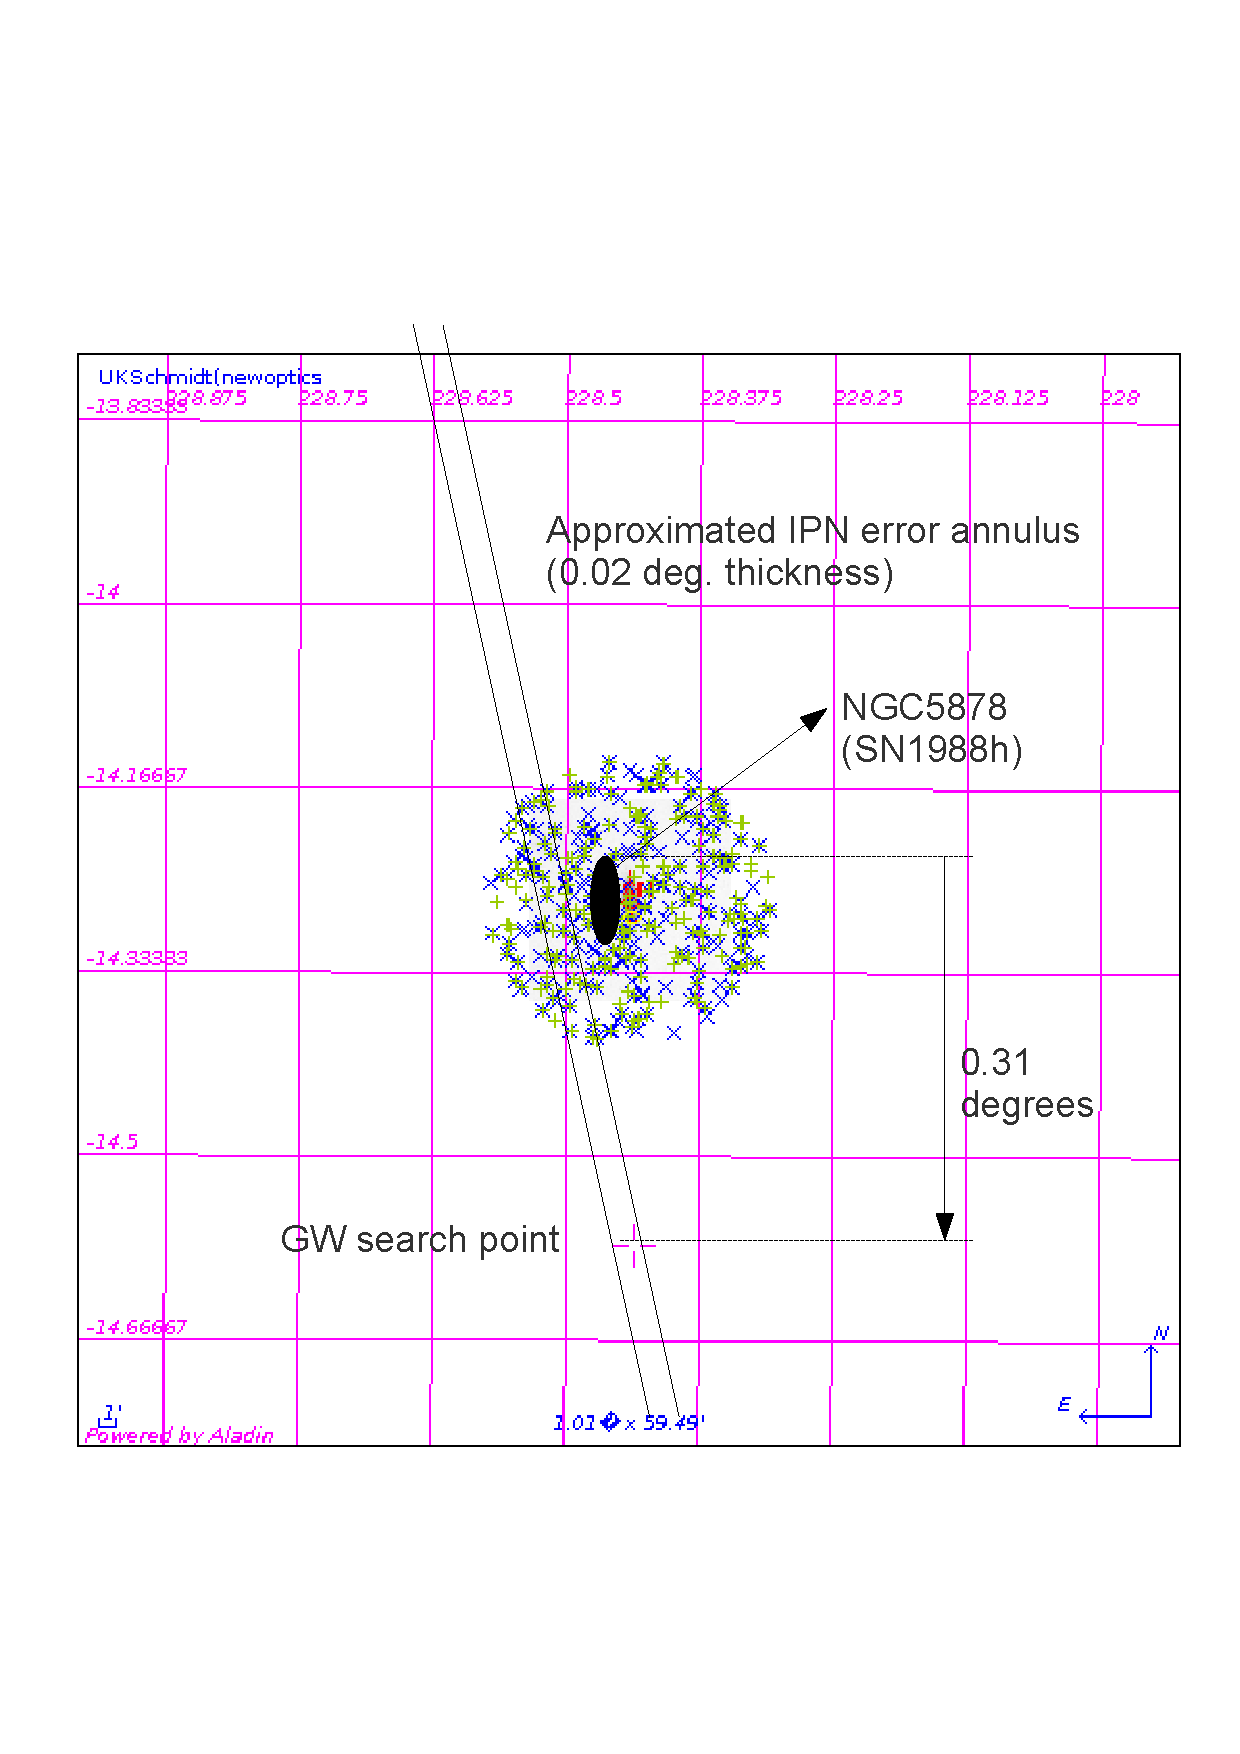
\includegraphics[scale=0.4]{Images/070321_search_point_NGC5878.pdf}
\end{minipage}
\caption{(Left figure) GRB070414 and nearby galaxy PGC004601 (Andromeda II): the IPN annulus intersects the outer regions of the galaxy error box. The GRB search point is located at RA=18.7719194 degrees, dec=33.5563965 degrees, with the galaxy center at RA=19.12407 degrees, dec=33.41910 degrees and galactic apparent size of 3.6$\times$2.52 arcminutes. $x$--axis represents RA and $y$--axis represents dec in J2000d degrees \cite{gwgc, ned}. (Right figure) GRB070321 and nearby galaxy NGC5878 (SN1988h): unfortunately, the IPN annulus does not intersect the outer regions of the galaxy error box. The GRB search point is located at RA=228.4346539, dec=-14.5788967 degrees, with the galaxy center at RA=228.440458, dec=-14.269833 and galactic apparent size of 3.5$\times$1.4 arcminutes. $x$--axis represents RA and $y$--axis represents dec in J2000d degrees \cite{gwgc, ned}.}
\label{ipngalaxies_search_point}
%\end{minipage}
\end{figure}

\section{Conclusion}
\label{sec:conclusion}

A search for gravitational waves coincident with gamma-ray bursts localized by the InterPlanetary Network during the S5/VSR1 science runs of LIGO and Virgo has been performed with results summarized in Table \ref{tab:ipn_grb_results}. In total, 12 short GRBs were analyzed, with data from multiple GW detectors, using the templated coherent method described in detail in \cite{Harry:2010fr}. This search represents a focused search that looked for CBC signals from the merger of two compact objects (either NS--NS or NS--BH), as expected for short GRBs, see Chapter \ref{Chapter Two} and references therein. No gravitational wave was detected in coincidence with a GRB.  Lower limits on the distance were set for each GRB and each of the two progenitor models: for the NS--NS progenitor model the median distance (at $30^\circ$ jet opening angle) is 18 Mpc and the mean distance is 17 Mpc; for the NS--BH progenitor model the median distance (at $30^\circ$ jet opening angle) is 31 Mpc and the mean distance is 31 Mpc. Possible host galaxies have been identified for two bursts: their positional error boxes marginally overlap two nearby galaxy error regions. Chances are small that these galaxies are indeed hosts for the GRBs, given both typical much larger redshifts for short bursts and the extended nature of the IPN error boxes.

The analysis process for the S5/VSR1 IPN--detected GRBs is not yet complete: we will need to analyze the remainder of 6 bursts with available GW data from H1H2--only. Furthermore, we will need to analyze the GW data around the IPN--detected bursts during S6/VSR2 and 3. When this will have finished, full results will be published in a scientific article.

\vspace{25mm}

\begin{table}[htb]
\begin{center}

Results for 12 short IPN GRBs with $\Delta A < 100 ~\mathrm{deg}^2$ and non--H1H2--only detector data

\begin{tabular}{*{6}{l}}
\hline
GRB&IPN&GW&UTC&Dist.&Dist.\\
Name&&&time&NS--NS&NS--BH\\
\hline
060103&MO/I &H1H2L1&Jan 03 2006 08:42:17& 5.2 & 9.2 \\
060107&K/MO/S&H1H2L1&Jan 07 2006 01:54:40& 21.7 & 37.6 \\
060203&K/MO/H&H1H2L1&Feb 03 2006 07:28:58& 5.7 & 10.3 \\ 
060415B&K/MO/S&H1H2L1&Apr 15 2006 18:14:44& 13.2 & 23.7\\
060522C&S/K/MO&H1H2L1&May 22 2006 10:10:19& 27.6 & 44.4\\ 
060708B&H/K/MO&H1H2L1&Jul 08 2006 04:30:38& 17.1 & 26.5 \\
060930A&K/MO&H1H2L1&Sept 30 2006 02:30:11& 17.8 & 33.3\\
061006A&K/MO/S&H1H2L1&Oct 06 2006 08:43:38& 26.6 & 47.3 \\
070321&I/K/MO/S&H1H2L1&Mar 21 2007 18:52:15& 20.1 & 36.1 \\
070516&I/K/M/S&H1H2L1&May 16 2007 20:41:24& 17.6 & 30.7 \\
070614&K/H&H1H2L1V1&Jun 14 2007 05:05:09& 17.0 & 29.1 \\ 
070915&Sw/I/M/K&H1H2L1V1&Sept 15 2007 08:34:48& 17.6 & 31.5 \\
\hline
\end{tabular}
\caption{\label{tab:shortGRB} The short S5/VSR1 IPN GRB sample analyzed at the time of this writing: 12 bursts with data from multiple non--H1H2--only GW detectors and well localized (error box area $\Delta A <$100$~\mathrm{deg}^2$); results show the 90\% exclusion distances (Mpc) for both possible progenitor models, either NS--NS or NS--BH for a jet--opening angle of 30$^\circ$. The IPN satellites that observed the bursts: S - Suzaku, Sw - \emph{Swift}, I - INTEGRAL, M - MESSENGER, MO - Mars Odyssey, K - Konus-WIND, H - HESSI (RHESSI).}
\end{center}
\label{tab:ipn_grb_results}
\end{table}

